\documentclass{article}
\usepackage[utf8]{inputenc}
\usepackage{natbib}
\usepackage{lineno}
\usepackage{graphicx}
\usepackage{float}
\usepackage{adjustbox}
\usepackage{dcolumn}
\usepackage{amsmath}
\usepackage{setspace}
\usepackage{authblk}
\usepackage{xr-hyper}
\usepackage[hidelinks]{hyperref}
\usepackage[top=1in, bottom=1in, left=1in, right=1in]{geometry}  
\usepackage[dvipsnames]{xcolor}

\usepackage[font=footnotesize, labelfont=bf]{caption}

%%%%%%%%%%%%%%%%%%%%%%%%%%%%%%%%%%%%%%%%%%%%%%%%%%%%%%%%%%%%%%%%%
\begin{document}

% --------------------------
\thispagestyle{empty}
\begin{center}
~~ \\ 
\bigskip 
\bigskip 
\bigskip 
\bigskip 
\bigskip 
\bigskip 
\bigskip 
\bigskip 
\bigskip 
\bigskip 
\bigskip 
\bigskip 
\bigskip 
\bigskip 
    \Huge The Evolution of the COVID-19 Pandemic Through the Lens of Google Searches \\
    \bigskip
    \bigskip
    \bigskip
    \Huge Main Text: Figures and Tables
\end{center}
    \bigskip
    \bigskip
    \bigskip
    \bigskip
    \bigskip
    \bigskip
    \bigskip
    \bigskip
    \bigskip
    \bigskip
    \bigskip
    \bigskip
    \bigskip
    \bigskip
    \bigskip
    \bigskip
    \bigskip
    \bigskip
    \bigskip
    \bigskip
    \bigskip
    \bigskip
    \bigskip

\newpage

\begin{figure*}[t]
    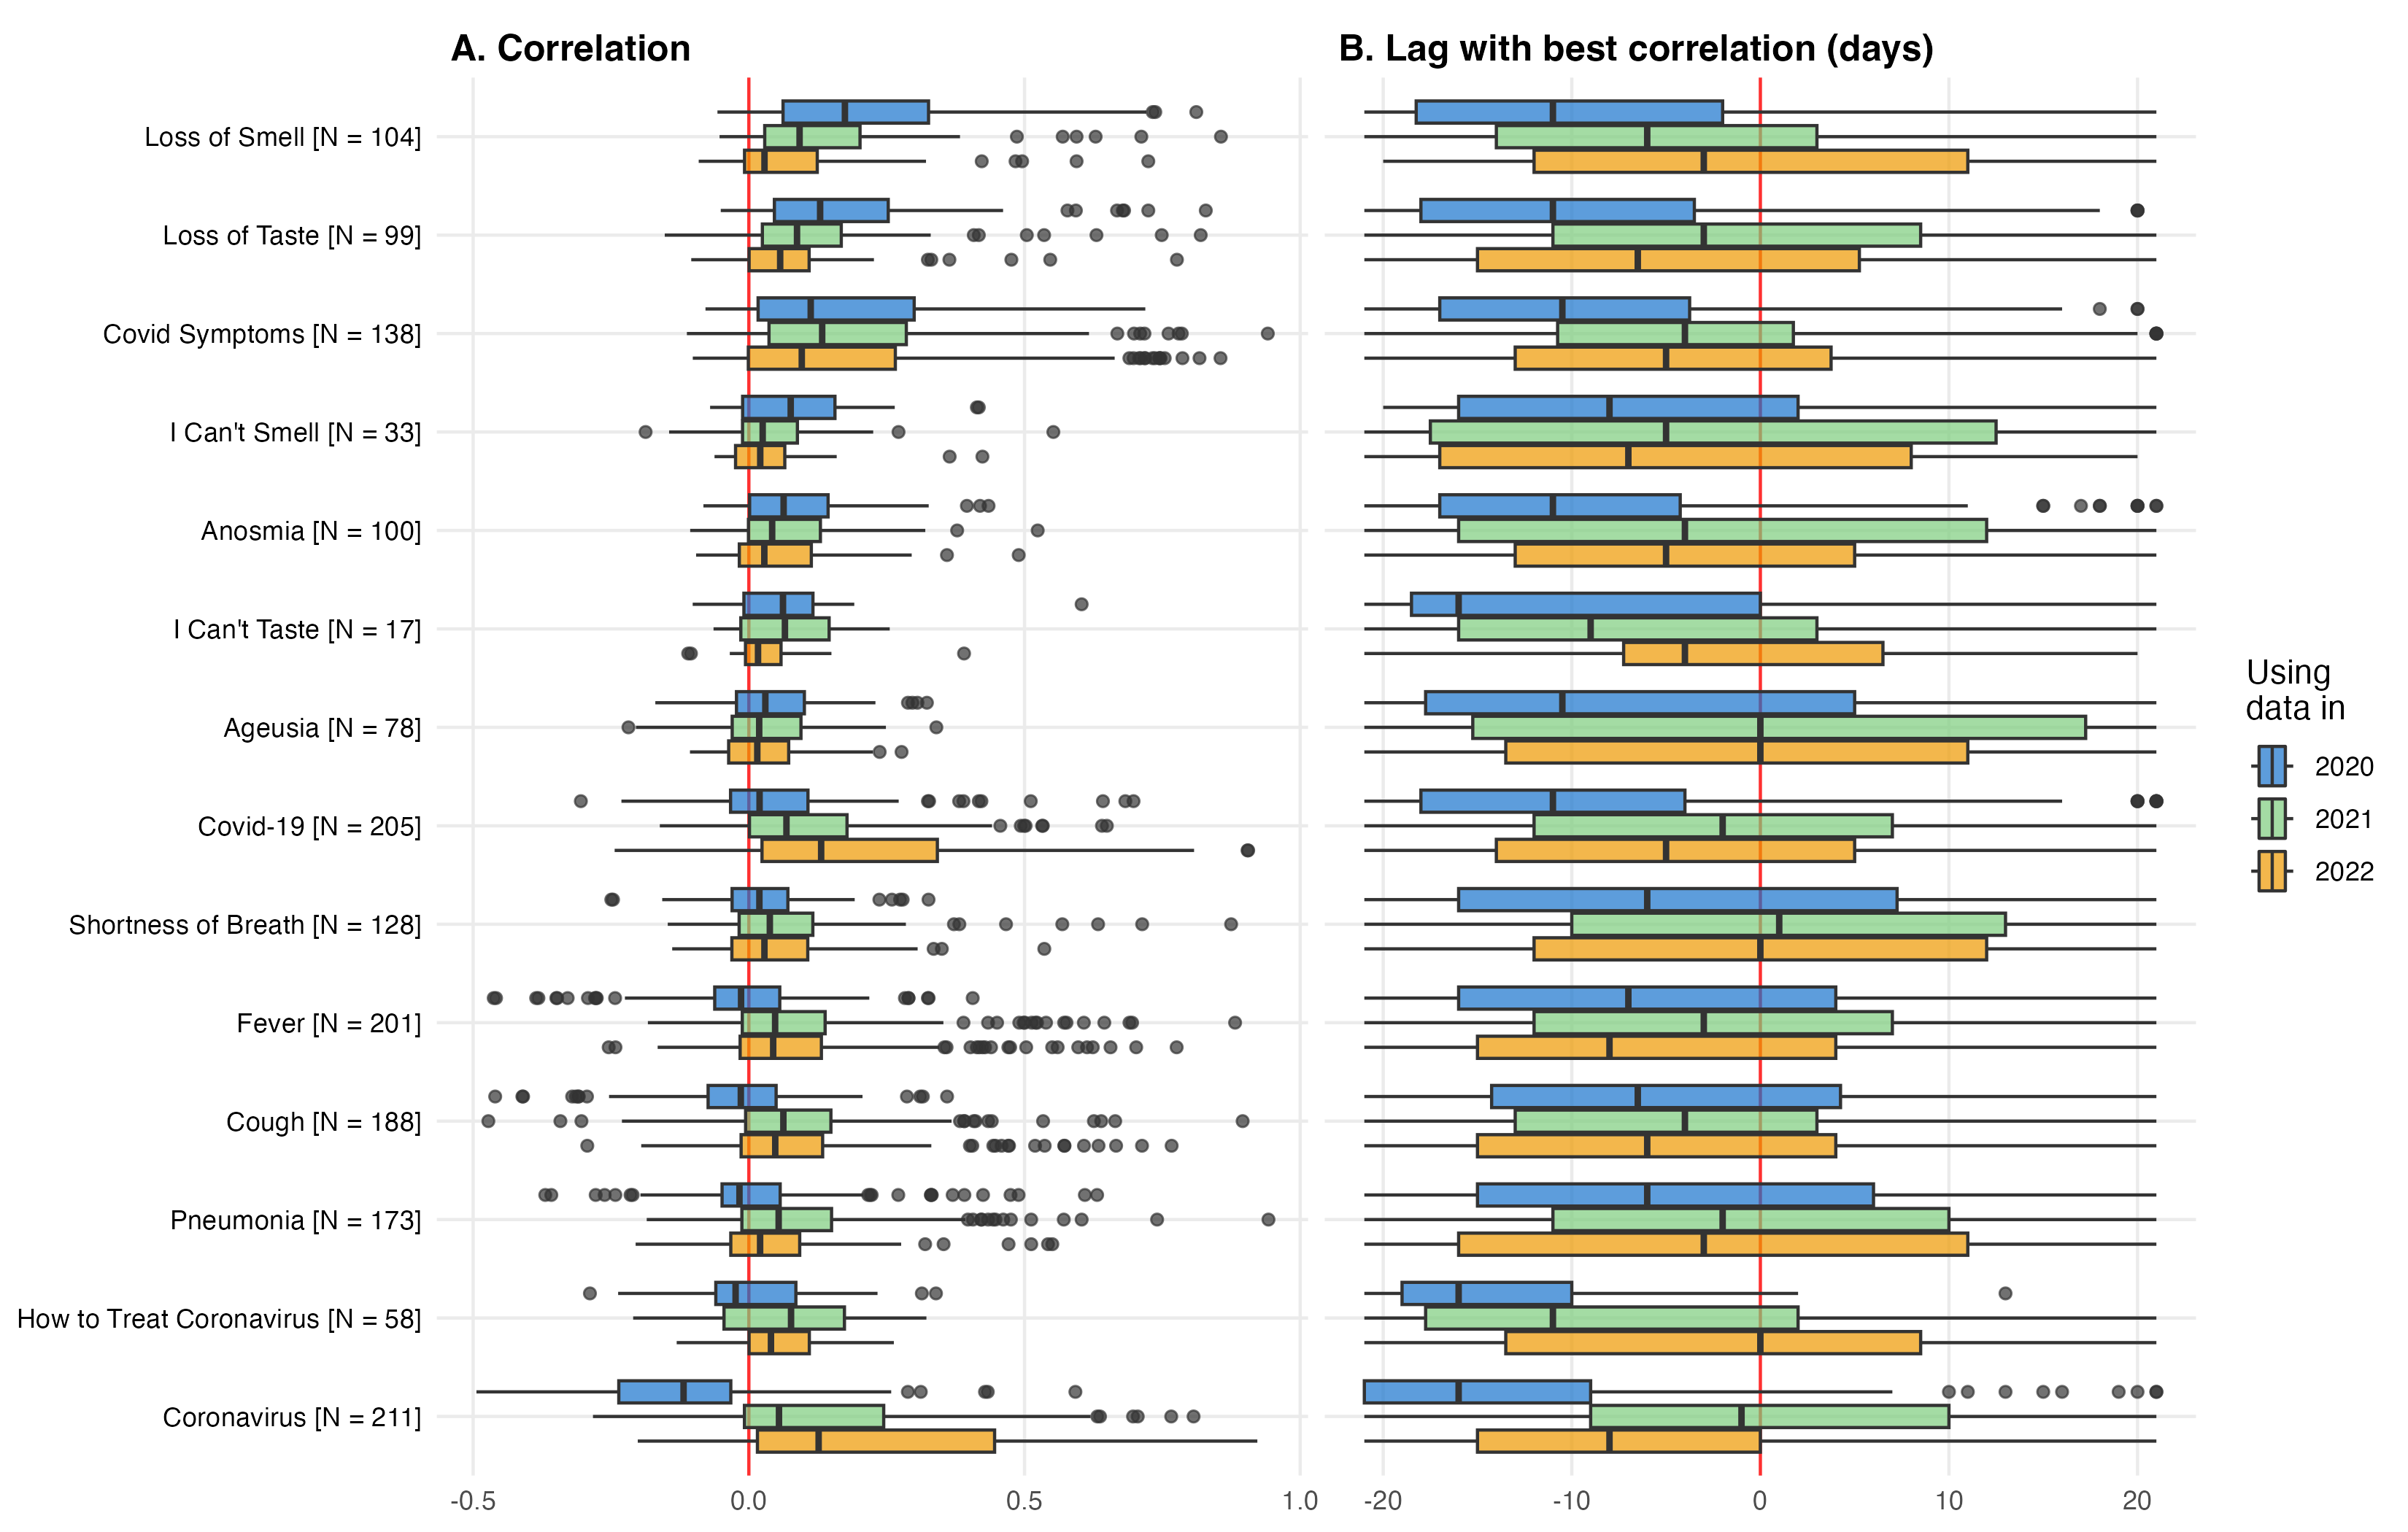
\includegraphics[width=1\textwidth]{figures/cor_lag_fig.png}
    \caption{Search interest correlating with and anticipating COVID-19 cases. Panel A shows the correlation between search interest and \textcolor{black}{reported} COVID-19 cases. Panel B shows the lead/lad value of COVID-19 cases that produced the highest correlation with search interest. \textcolor{black}{`N' indicates the number of countries with available data.} The boxplots include: center line, median; box limits, upper and lower quartiles; whiskers, 1.5x interquartile range; points beyond whiskers, outliers.}
    \label{fig:corlag_figure}
\end{figure*}

\begin{figure*}[t]
    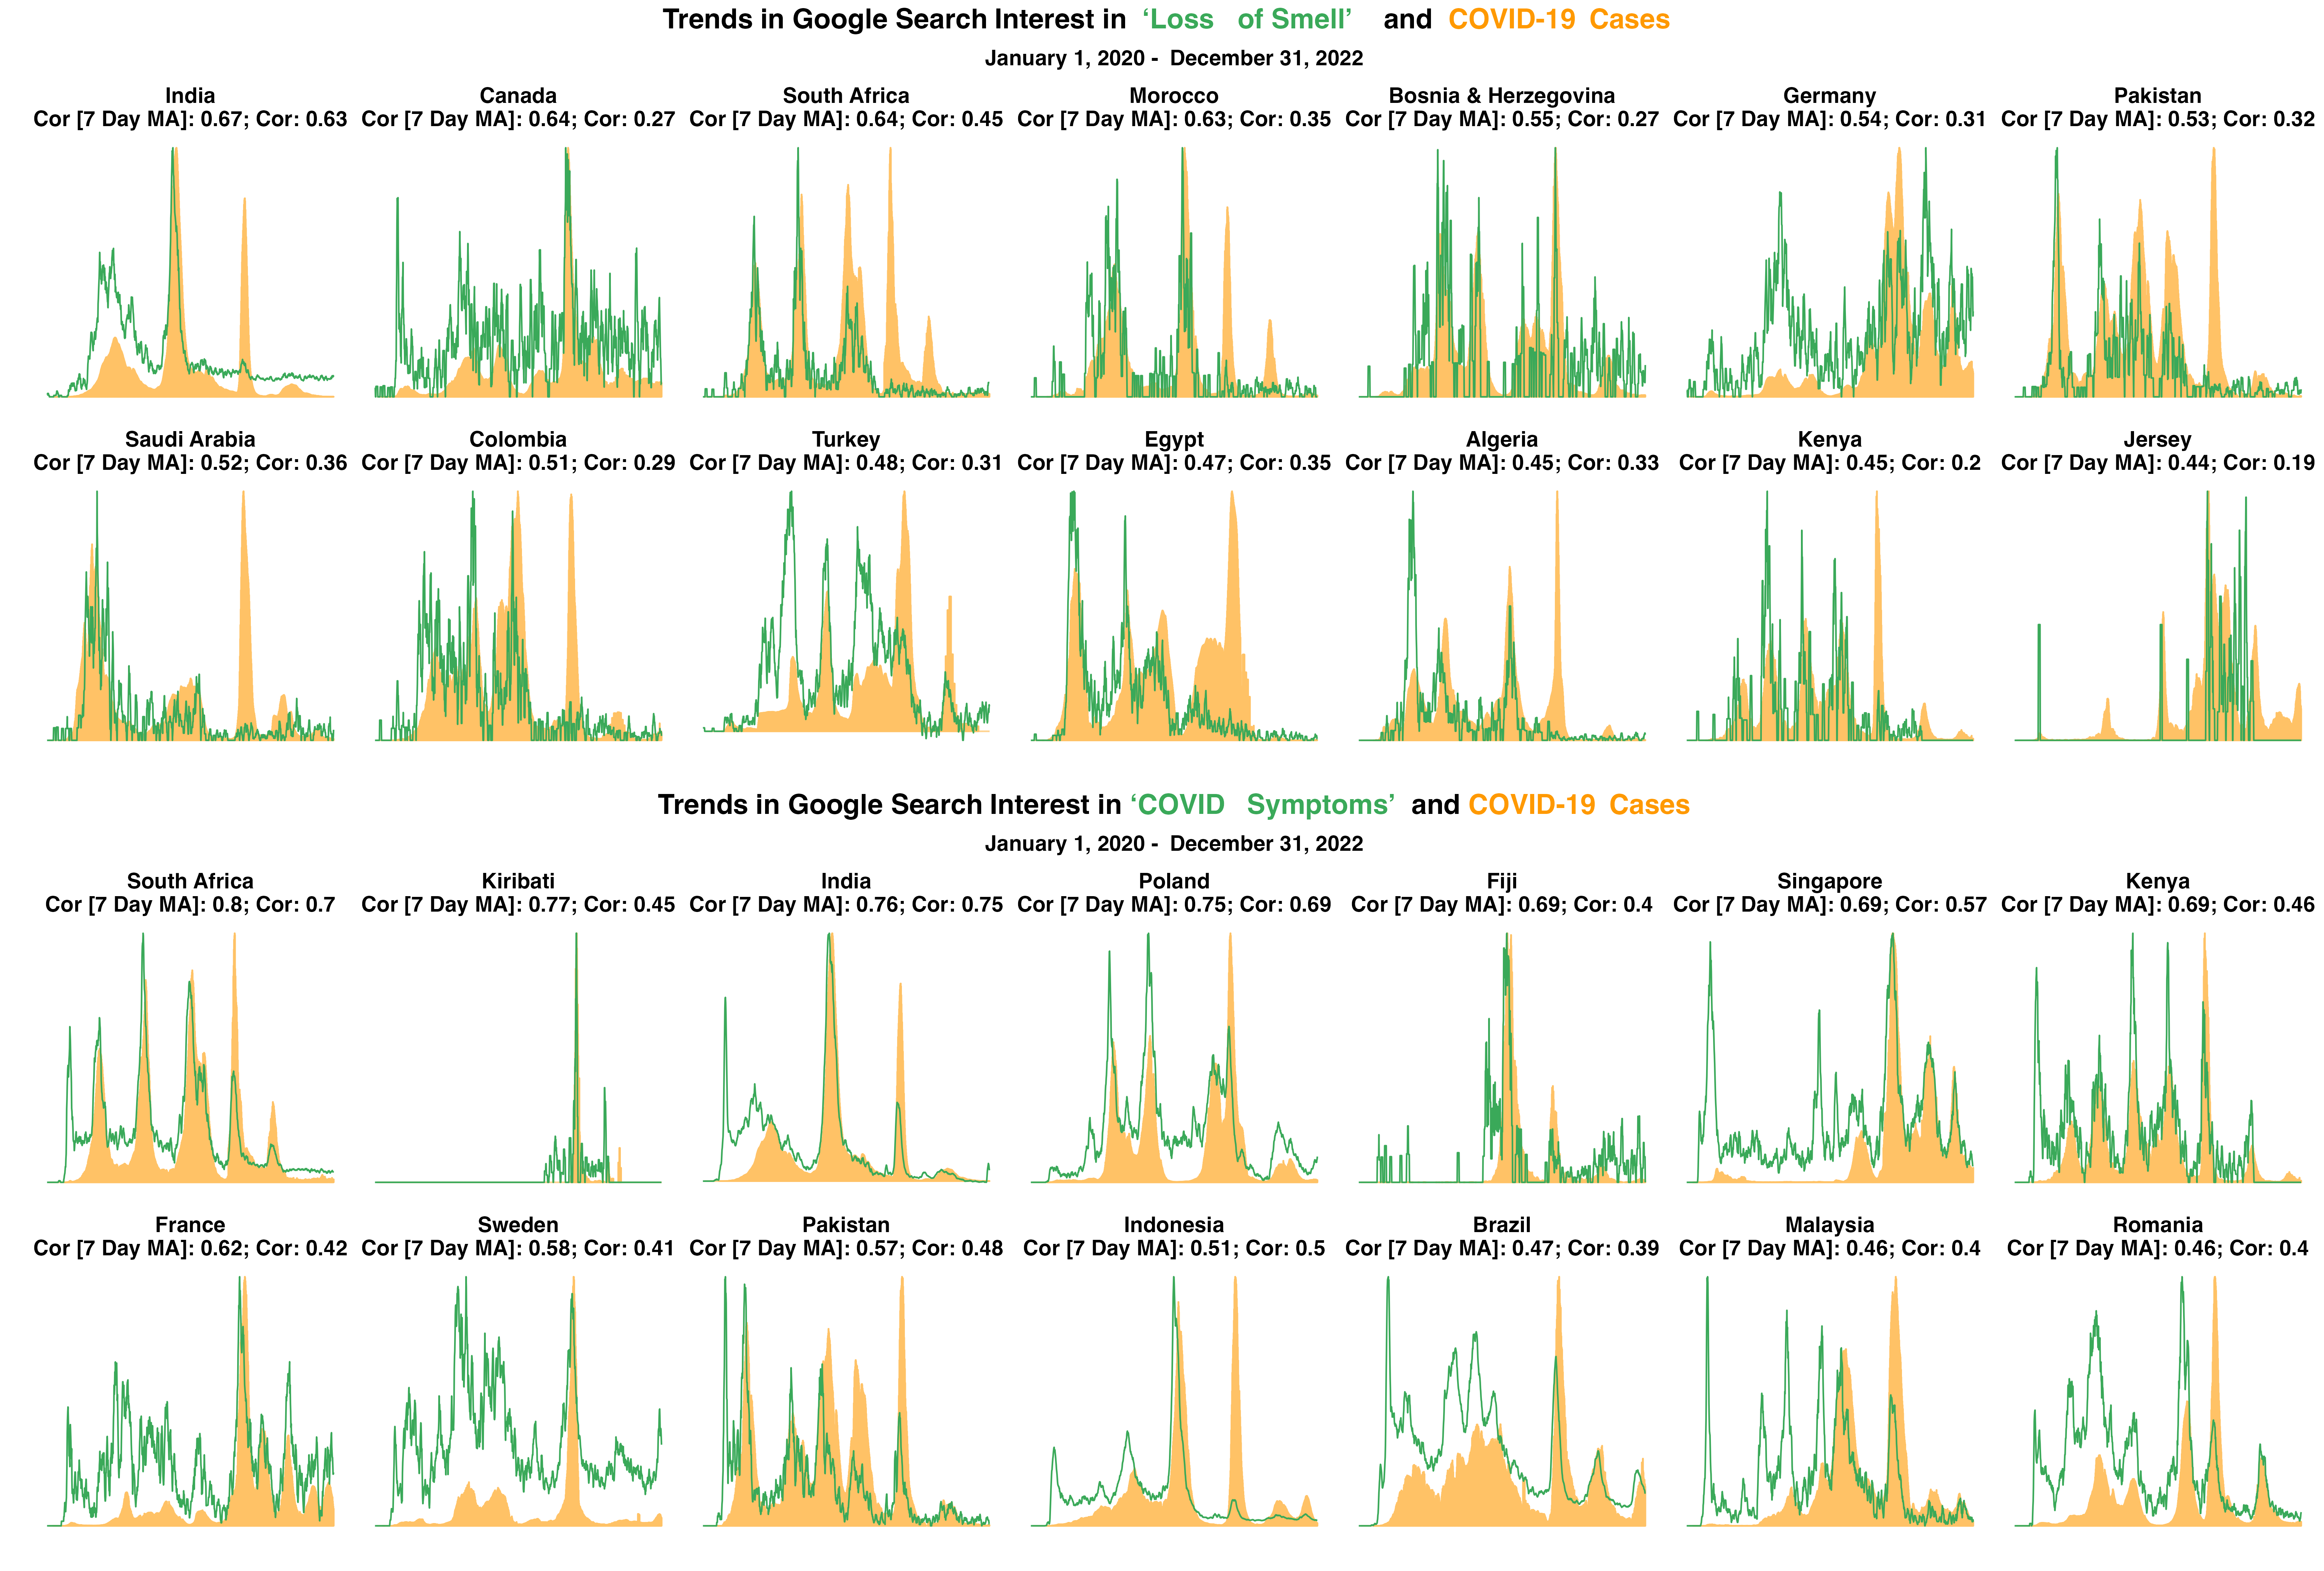
\includegraphics[width=1\textwidth]{figures/cases_vs_loss_of_smell_covid_symptoms_trends_topcountries.png}
    \caption{Trends between \textcolor{black}{reported} COVID-19 cases and search interest in (1) ``Loss of Smell'' (top) and (2) ``COVID Symptoms'' for countries with the top correlations between cases and search interest. \textcolor{black}{To more clearly show trends, the seven-day moving averages of search interest and cases are shown.}}
    \label{fig:cor_trends_figure}
\end{figure*}

\setlength{\tabcolsep}{4pt}
\begin{table*}[t!]
\centering
\caption{Explaining correlation between search interest in loss of smell and COVID-19 cases, using data from 2020 and 2021}

% Table created by stargazer v.5.2.3 by Marek Hlavac, Social Policy Institute. E-mail: marek.hlavac at gmail.com
% Date and time: Fri, Oct 13, 2023 - 09:00:08
% Requires LaTeX packages: dcolumn 
\begin{tabular}{@{\extracolsep{-15pt}}lD{.}{.}{-2} D{.}{.}{-2} D{.}{.}{-2} D{.}{.}{-2} D{.}{.}{-2} D{.}{.}{-2} D{.}{.}{-2} D{.}{.}{-2} } 
\\[-1.8ex]\hline 
\hline \\[-1.8ex] 
 & \multicolumn{8}{c}{\textit{Dependent variable:}} \\ 
\cline{2-9} 
\\[-1.8ex] & \multicolumn{8}{c}{Correlation} \\ 
\\[-1.8ex] & \multicolumn{1}{c}{(1)} & \multicolumn{1}{c}{(2)} & \multicolumn{1}{c}{(3)} & \multicolumn{1}{c}{(4)} & \multicolumn{1}{c}{(5)} & \multicolumn{1}{c}{(6)} & \multicolumn{1}{c}{(7)} & \multicolumn{1}{c}{(8)}\\ 
\hline \\[-1.8ex] 
 Total COVID-19 Cases, log & 0.02^{***} &  &  &  &  &  & 0.03^{***} & 0.03^{***} \\ 
  & (0.01) &  &  &  &  &  & (0.01) & (0.01) \\ 
  Per Pop. Using Internet &  & 0.0000 &  &  &  &  &  & 0.0002 \\ 
  &  & (0.001) &  &  &  &  &  & (0.002) \\ 
  Mobile Cell Sub. per 100 &  &  & 0.0000 &  &  &  &  & 0.0002 \\ 
  &  &  & (0.0005) &  &  &  &  & (0.001) \\ 
  GDP Per Cap, Log &  &  &  & -0.004 &  &  & -0.04 & -0.04 \\ 
  &  &  &  & (0.01) &  &  & (0.03) & (0.04) \\ 
  Low Income &  &  &  &  & -0.01 &  & 0.03 & 0.03 \\ 
  &  &  &  &  & (0.06) &  & (0.13) & (0.13) \\ 
  Lower Middle Income &  &  &  &  & 0.05 &  & 0.04 & 0.04 \\ 
  &  &  &  &  & (0.04) &  & (0.09) & (0.09) \\ 
  Upper Middle Income &  &  &  &  & 0.005 &  & 0.01 & 0.01 \\ 
  &  &  &  &  & (0.04) &  & (0.06) & (0.06) \\ 
  Europe and Central Asia &  &  &  &  &  & -0.03 & -0.01 & -0.01 \\ 
  &  &  &  &  &  & (0.05) & (0.05) & (0.06) \\ 
  Latin America and Caribbean &  &  &  &  &  & -0.06 & -0.03 & -0.03 \\ 
  &  &  &  &  &  & (0.06) & (0.06) & (0.06) \\ 
  Middle East and North Africa &  &  &  &  &  & 0.02 & 0.04 & 0.04 \\ 
  &  &  &  &  &  & (0.06) & (0.06) & (0.06) \\ 
  North America &  &  &  &  &  & 0.33^{***} & 0.34^{***} & 0.35^{***} \\ 
  &  &  &  &  &  & (0.11) & (0.11) & (0.12) \\ 
  South Asia &  &  &  &  &  & 0.20^{**} & 0.14 & 0.15 \\ 
  &  &  &  &  &  & (0.10) & (0.10) & (0.10) \\ 
  Sub-Saharan Africa &  &  &  &  &  & -0.07 & -0.06 & -0.06 \\ 
  &  &  &  &  &  & (0.06) & (0.06) & (0.07) \\ 
  Constant & -0.18^{*} & 0.13^{***} & 0.13^{**} & 0.17 & 0.12^{***} & 0.15^{***} & 0.05 & 0.05 \\ 
  & (0.10) & (0.05) & (0.06) & (0.11) & (0.03) & (0.05) & (0.34) & (0.36) \\ 
 \hline \\[-1.8ex] 
Observations & \multicolumn{1}{c}{112} & \multicolumn{1}{c}{106} & \multicolumn{1}{c}{110} & \multicolumn{1}{c}{107} & \multicolumn{1}{c}{109} & \multicolumn{1}{c}{112} & \multicolumn{1}{c}{107} & \multicolumn{1}{c}{105} \\ 
Adjusted R$^{2}$ & \multicolumn{1}{c}{0.08} & \multicolumn{1}{c}{-0.01} & \multicolumn{1}{c}{-0.01} & \multicolumn{1}{c}{-0.01} & \multicolumn{1}{c}{-0.01} & \multicolumn{1}{c}{0.14} & \multicolumn{1}{c}{0.22} & \multicolumn{1}{c}{0.20} \\ 
\hline 
\hline \\[-1.8ex] 
\end{tabular} 
 \\
\flushleft $^{*}$p$<$0.1; $^{**}$p$<$0.05; $^{***}$p$<$0.01
\label{tab:cor_reg_table}
\end{table*}

\setlength{\tabcolsep}{4pt}
\begin{table*}[t!]
\centering
\caption{Explaining the lead/lag value that produced the highest correlation between search interest in loss of smell and COVID-19 cases, using data from 2020 and 2021}

% Table created by stargazer v.5.2.3 by Marek Hlavac, Social Policy Institute. E-mail: marek.hlavac at gmail.com
% Date and time: Fri, Oct 13, 2023 - 09:00:09
% Requires LaTeX packages: dcolumn 
\begin{tabular}{@{\extracolsep{-15pt}}lD{.}{.}{-2} D{.}{.}{-2} D{.}{.}{-2} D{.}{.}{-2} D{.}{.}{-2} D{.}{.}{-2} D{.}{.}{-2} D{.}{.}{-2} } 
\\[-1.8ex]\hline 
\hline \\[-1.8ex] 
 & \multicolumn{8}{c}{\textit{Dependent variable:}} \\ 
\cline{2-9} 
\\[-1.8ex] & \multicolumn{8}{c}{Best Lag} \\ 
\\[-1.8ex] & \multicolumn{1}{c}{(1)} & \multicolumn{1}{c}{(2)} & \multicolumn{1}{c}{(3)} & \multicolumn{1}{c}{(4)} & \multicolumn{1}{c}{(5)} & \multicolumn{1}{c}{(6)} & \multicolumn{1}{c}{(7)} & \multicolumn{1}{c}{(8)}\\ 
\hline \\[-1.8ex] 
 Total COVID-19 Cases, log & 0.07 &  &  &  &  &  & -0.33 & -0.44 \\ 
  & (0.52) &  &  &  &  &  & (0.69) & (0.71) \\ 
  Per Pop. Using Internet &  & 0.03 &  &  &  &  &  & 0.06 \\ 
  &  & (0.05) &  &  &  &  &  & (0.13) \\ 
  Mobile Cell Sub. per 100 &  &  & 0.06^{*} &  &  &  &  & 0.05 \\ 
  &  &  & (0.03) &  &  &  &  & (0.05) \\ 
  GDP Per Cap, Log &  &  &  & 0.56 &  &  & 0.19 & -1.13 \\ 
  &  &  &  & (0.90) &  &  & (2.51) & (2.96) \\ 
  Low Income &  &  &  &  & -4.99 &  & -14.11 & -12.75 \\ 
  &  &  &  &  & (4.15) &  & (9.49) & (9.74) \\ 
  Lower Middle Income &  &  &  &  & -1.36 &  & -5.06 & -4.74 \\ 
  &  &  &  &  & (2.87) &  & (6.57) & (6.65) \\ 
  Upper Middle Income &  &  &  &  & -1.44 &  & -0.63 & -1.48 \\ 
  &  &  &  &  & (2.80) &  & (4.33) & (4.45) \\ 
  Europe and Central Asia &  &  &  &  &  & 0.11 & -0.97 & -0.74 \\ 
  &  &  &  &  &  & (3.91) & (4.08) & (4.20) \\ 
  Latin America and Caribbean &  &  &  &  &  & -8.58^{**} & -9.92^{**} & -9.46^{**} \\ 
  &  &  &  &  &  & (4.07) & (4.31) & (4.38) \\ 
  Middle East and North Africa &  &  &  &  &  & -1.78 & -0.56 & -1.35 \\ 
  &  &  &  &  &  & (4.27) & (4.37) & (4.63) \\ 
  North America &  &  &  &  &  & 3.00 & 1.26 & 3.43 \\ 
  &  &  &  &  &  & (8.38) & (8.57) & (8.87) \\ 
  South Asia &  &  &  &  &  & 1.83 & 3.50 & 4.40 \\ 
  &  &  &  &  &  & (7.12) & (7.28) & (7.54) \\ 
  Sub-Saharan Africa &  &  &  &  &  & 3.50 & 8.26^{*} & 8.57^{*} \\ 
  &  &  &  &  &  & (4.13) & (4.84) & (5.08) \\ 
  Constant & -7.71 & -8.21^{**} & -13.41^{***} & -11.57 & -5.41^{***} & -5.50 & -0.32 & 3.58 \\ 
  & (7.15) & (3.22) & (3.99) & (8.01) & (1.98) & (3.42) & (25.51) & (26.78) \\ 
 \hline \\[-1.8ex] 
Observations & \multicolumn{1}{c}{112} & \multicolumn{1}{c}{106} & \multicolumn{1}{c}{110} & \multicolumn{1}{c}{107} & \multicolumn{1}{c}{109} & \multicolumn{1}{c}{112} & \multicolumn{1}{c}{107} & \multicolumn{1}{c}{105} \\ 
Adjusted R$^{2}$ & \multicolumn{1}{c}{-0.01} & \multicolumn{1}{c}{-0.01} & \multicolumn{1}{c}{0.02} & \multicolumn{1}{c}{-0.01} & \multicolumn{1}{c}{-0.01} & \multicolumn{1}{c}{0.09} & \multicolumn{1}{c}{0.12} & \multicolumn{1}{c}{0.12} \\ 
\hline 
\hline \\[-1.8ex] 
\end{tabular} 
 \\
\flushleft $^{*}$p$<$0.1; $^{**}$p$<$0.05; $^{***}$p$<$0.01
\label{tab:lag_reg_table}
\end{table*}

\begin{figure*}[t]
    \centering
    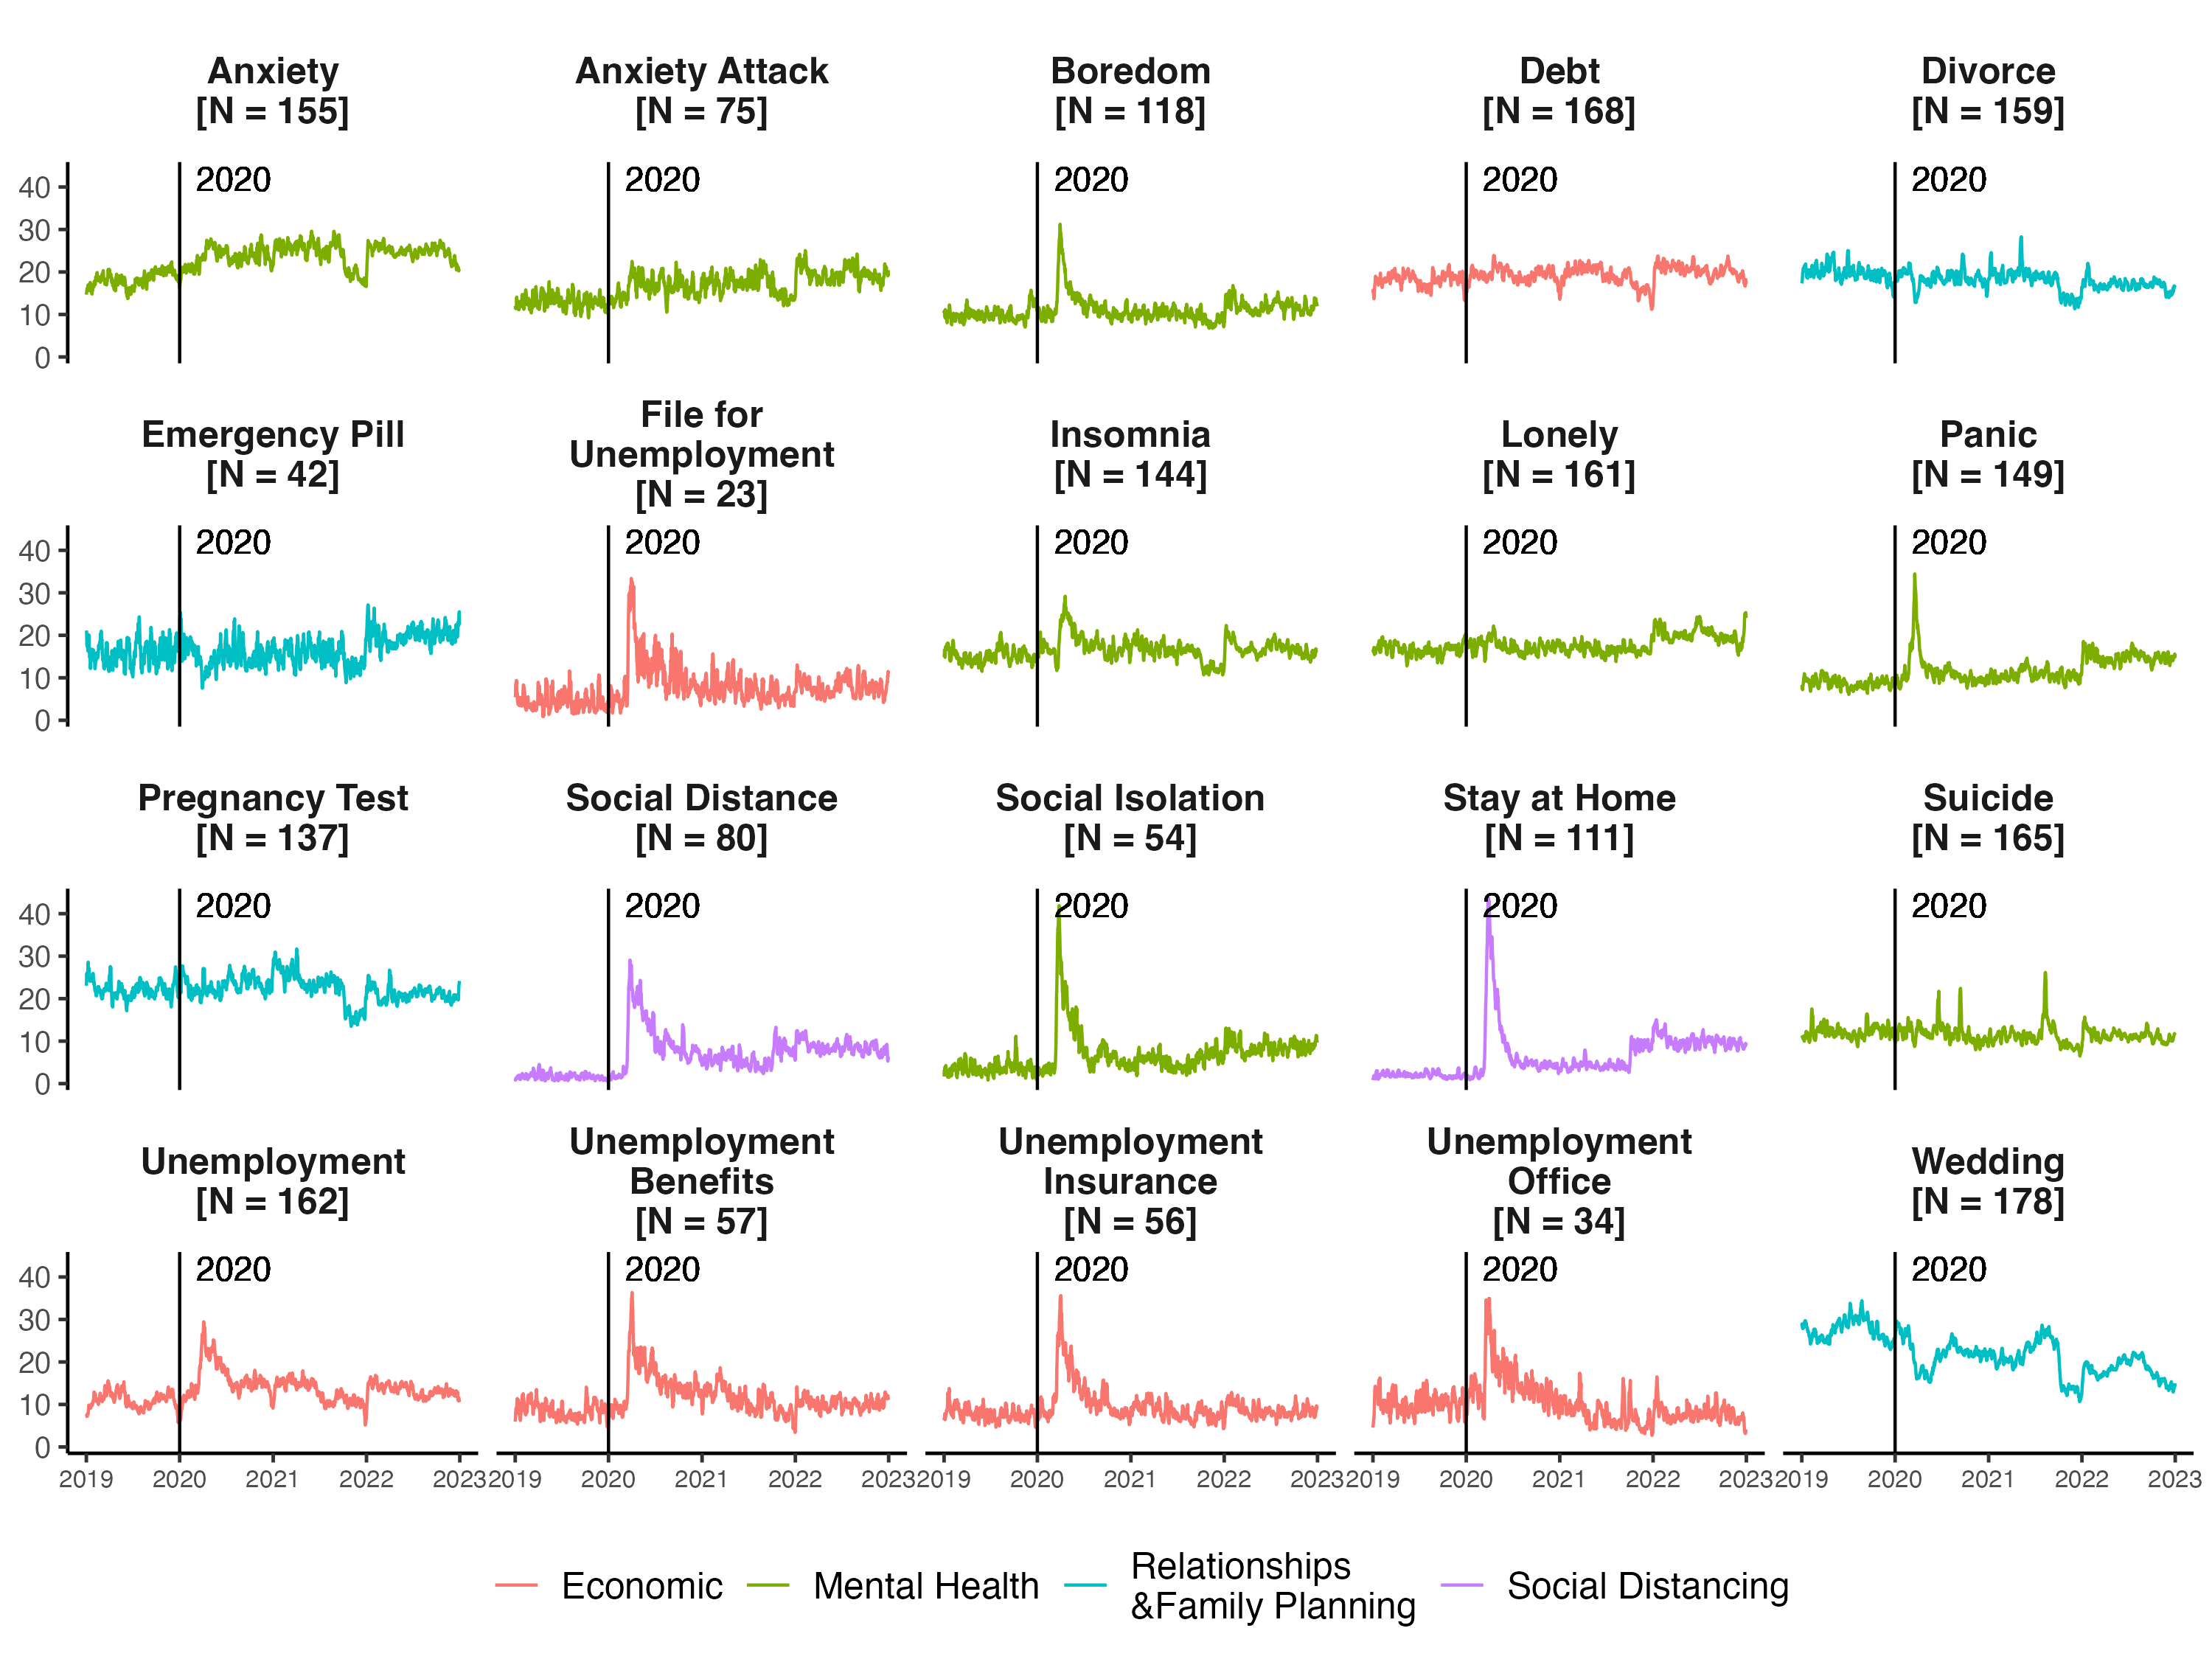
\includegraphics[width=0.85\textwidth]{figures/contain_long_trends.png}
    \caption{\textcolor{black}{Trends in search interest in social, economic, and mental health keywords from 2019 to 2022. To show trends more clearly, the seven-day moving average of search interest is shown. `N' indicates the number of countries with available data.}}
    \label{fig:contain_trends_long}
\end{figure*}

\begin{figure*}[t]
    \centering
    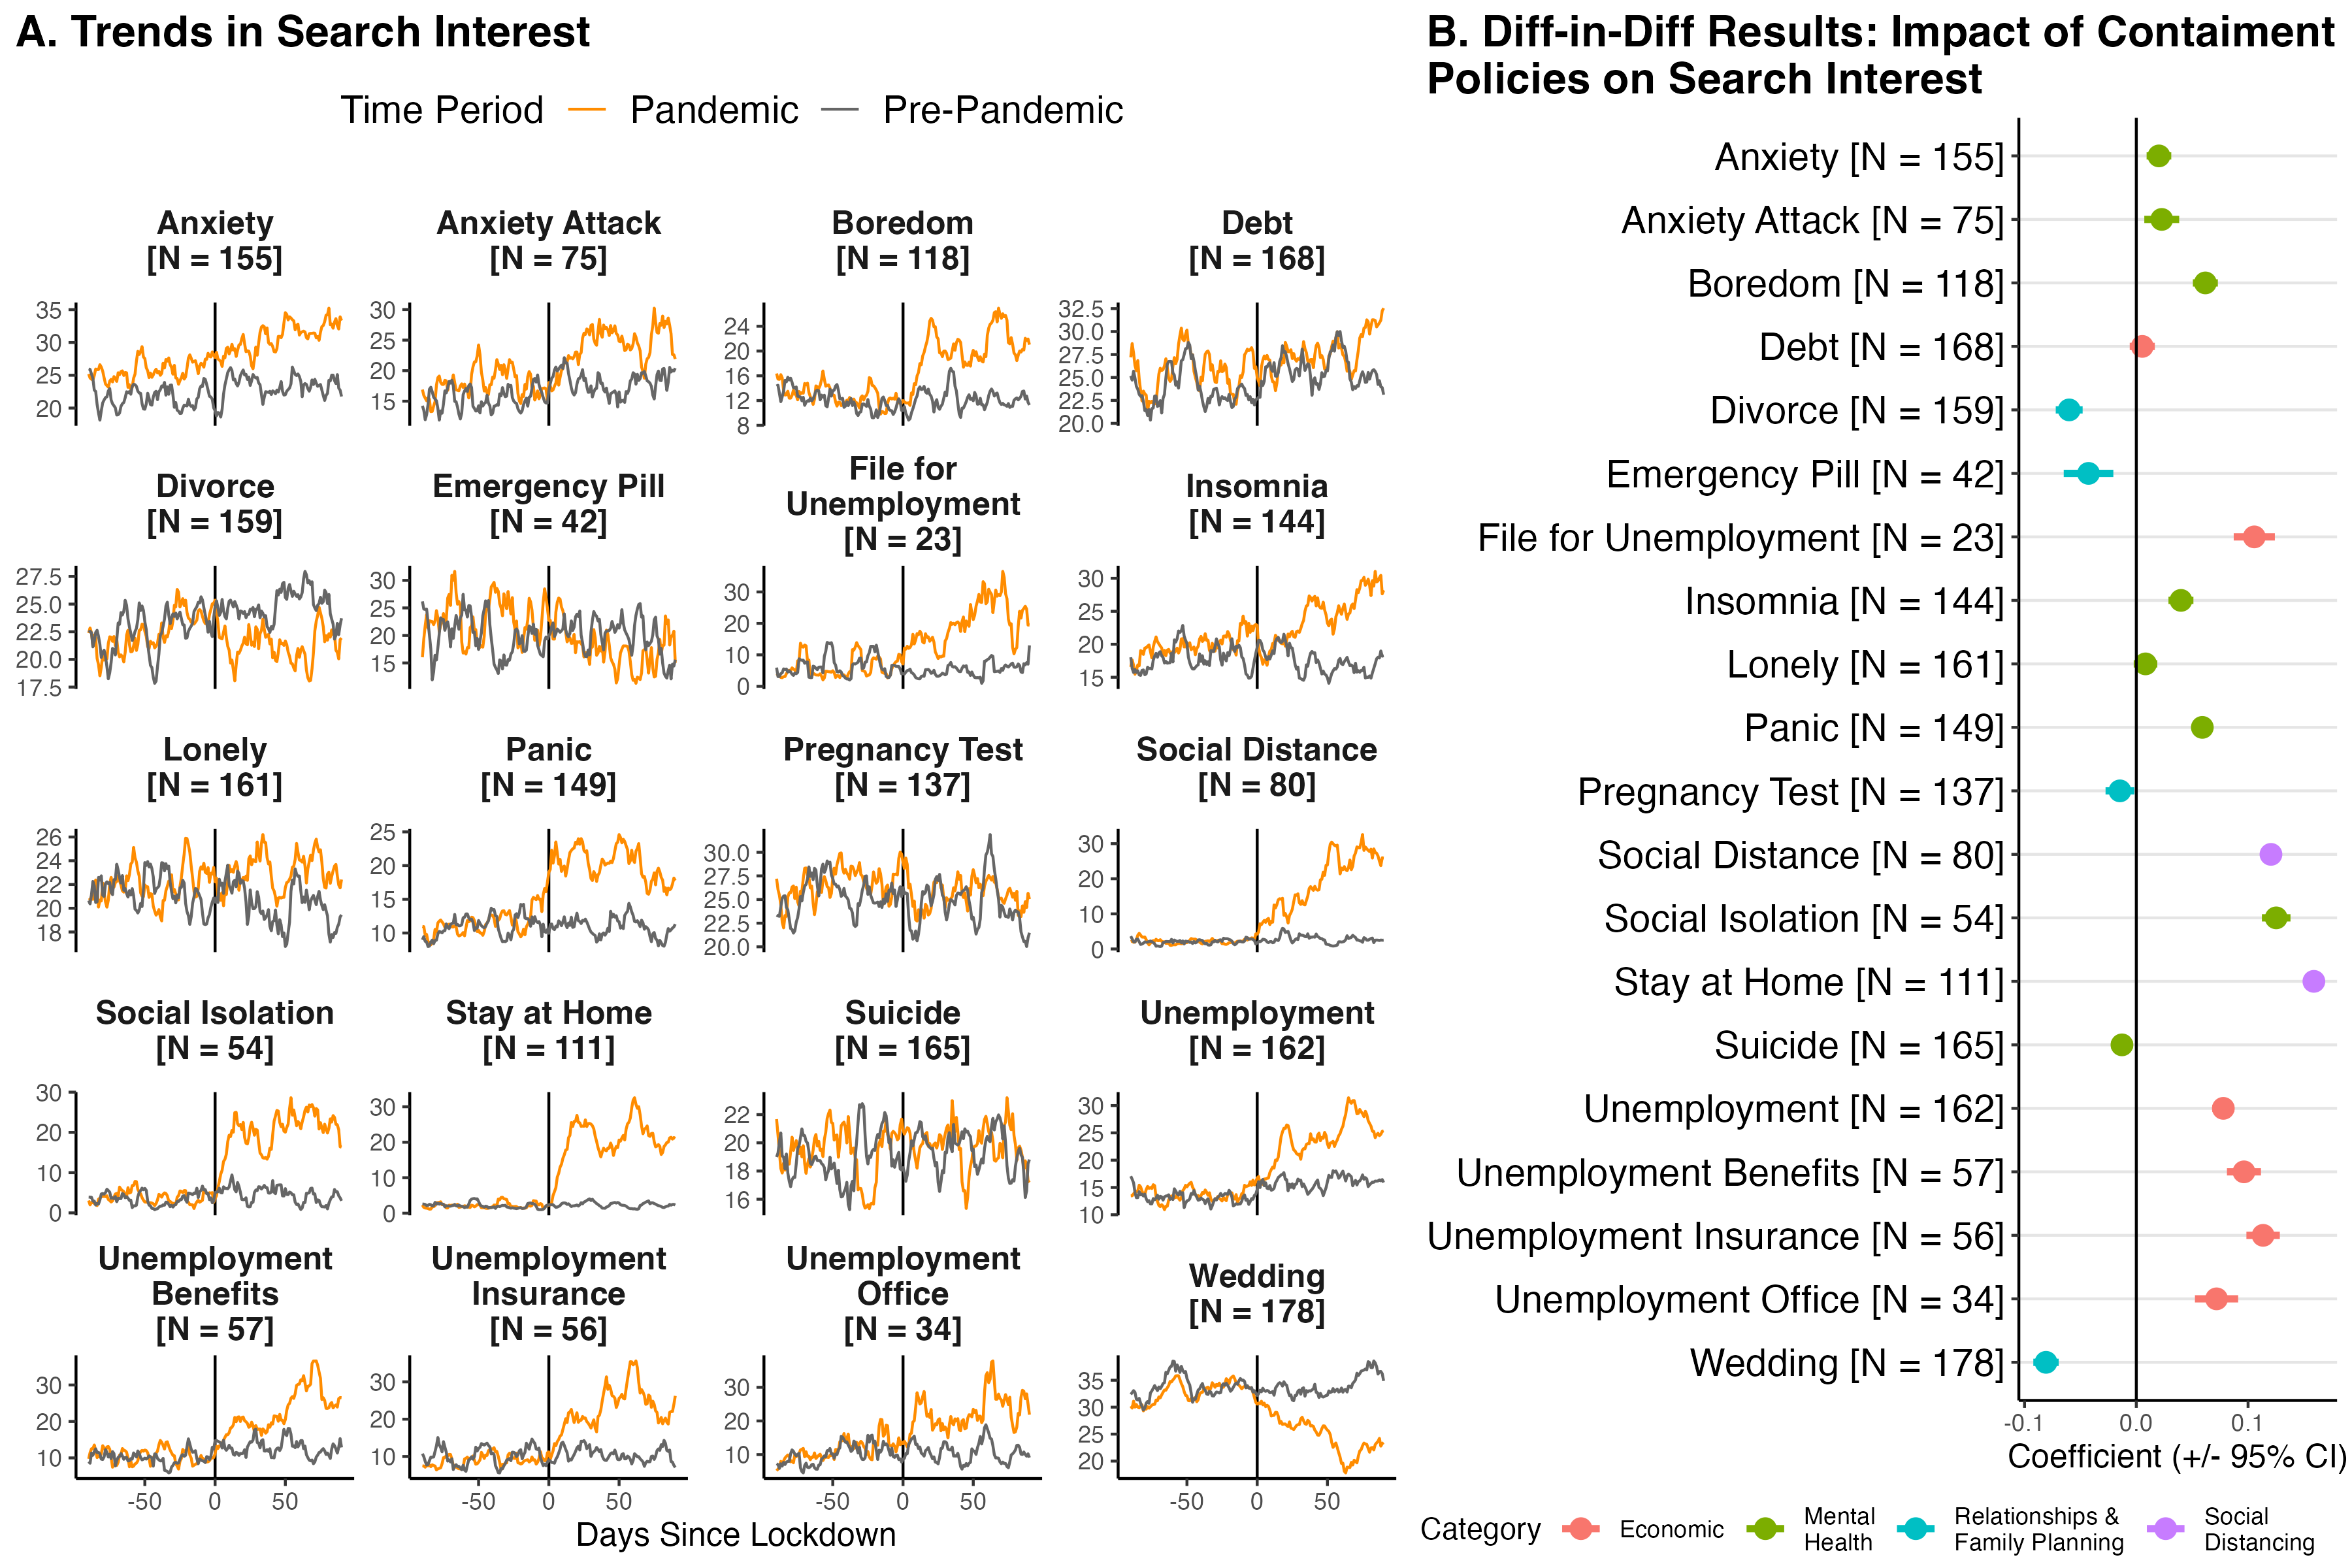
\includegraphics[width=0.85\textwidth]{figures/did_overall_90.png}
    \caption{\textcolor{black}{Association of COVID-19 policies and} search interest: results pooling all countries. Point estimates and 95\% confidence intervals are shown. \textcolor{black}{To show trends more clearly, the seven-day moving average of search interest is shown in panel A. `N' indicates the number of countries with available data.}}
    \label{fig:did_overall_90}
\end{figure*}

\begin{figure*}[!t]
    \centering
    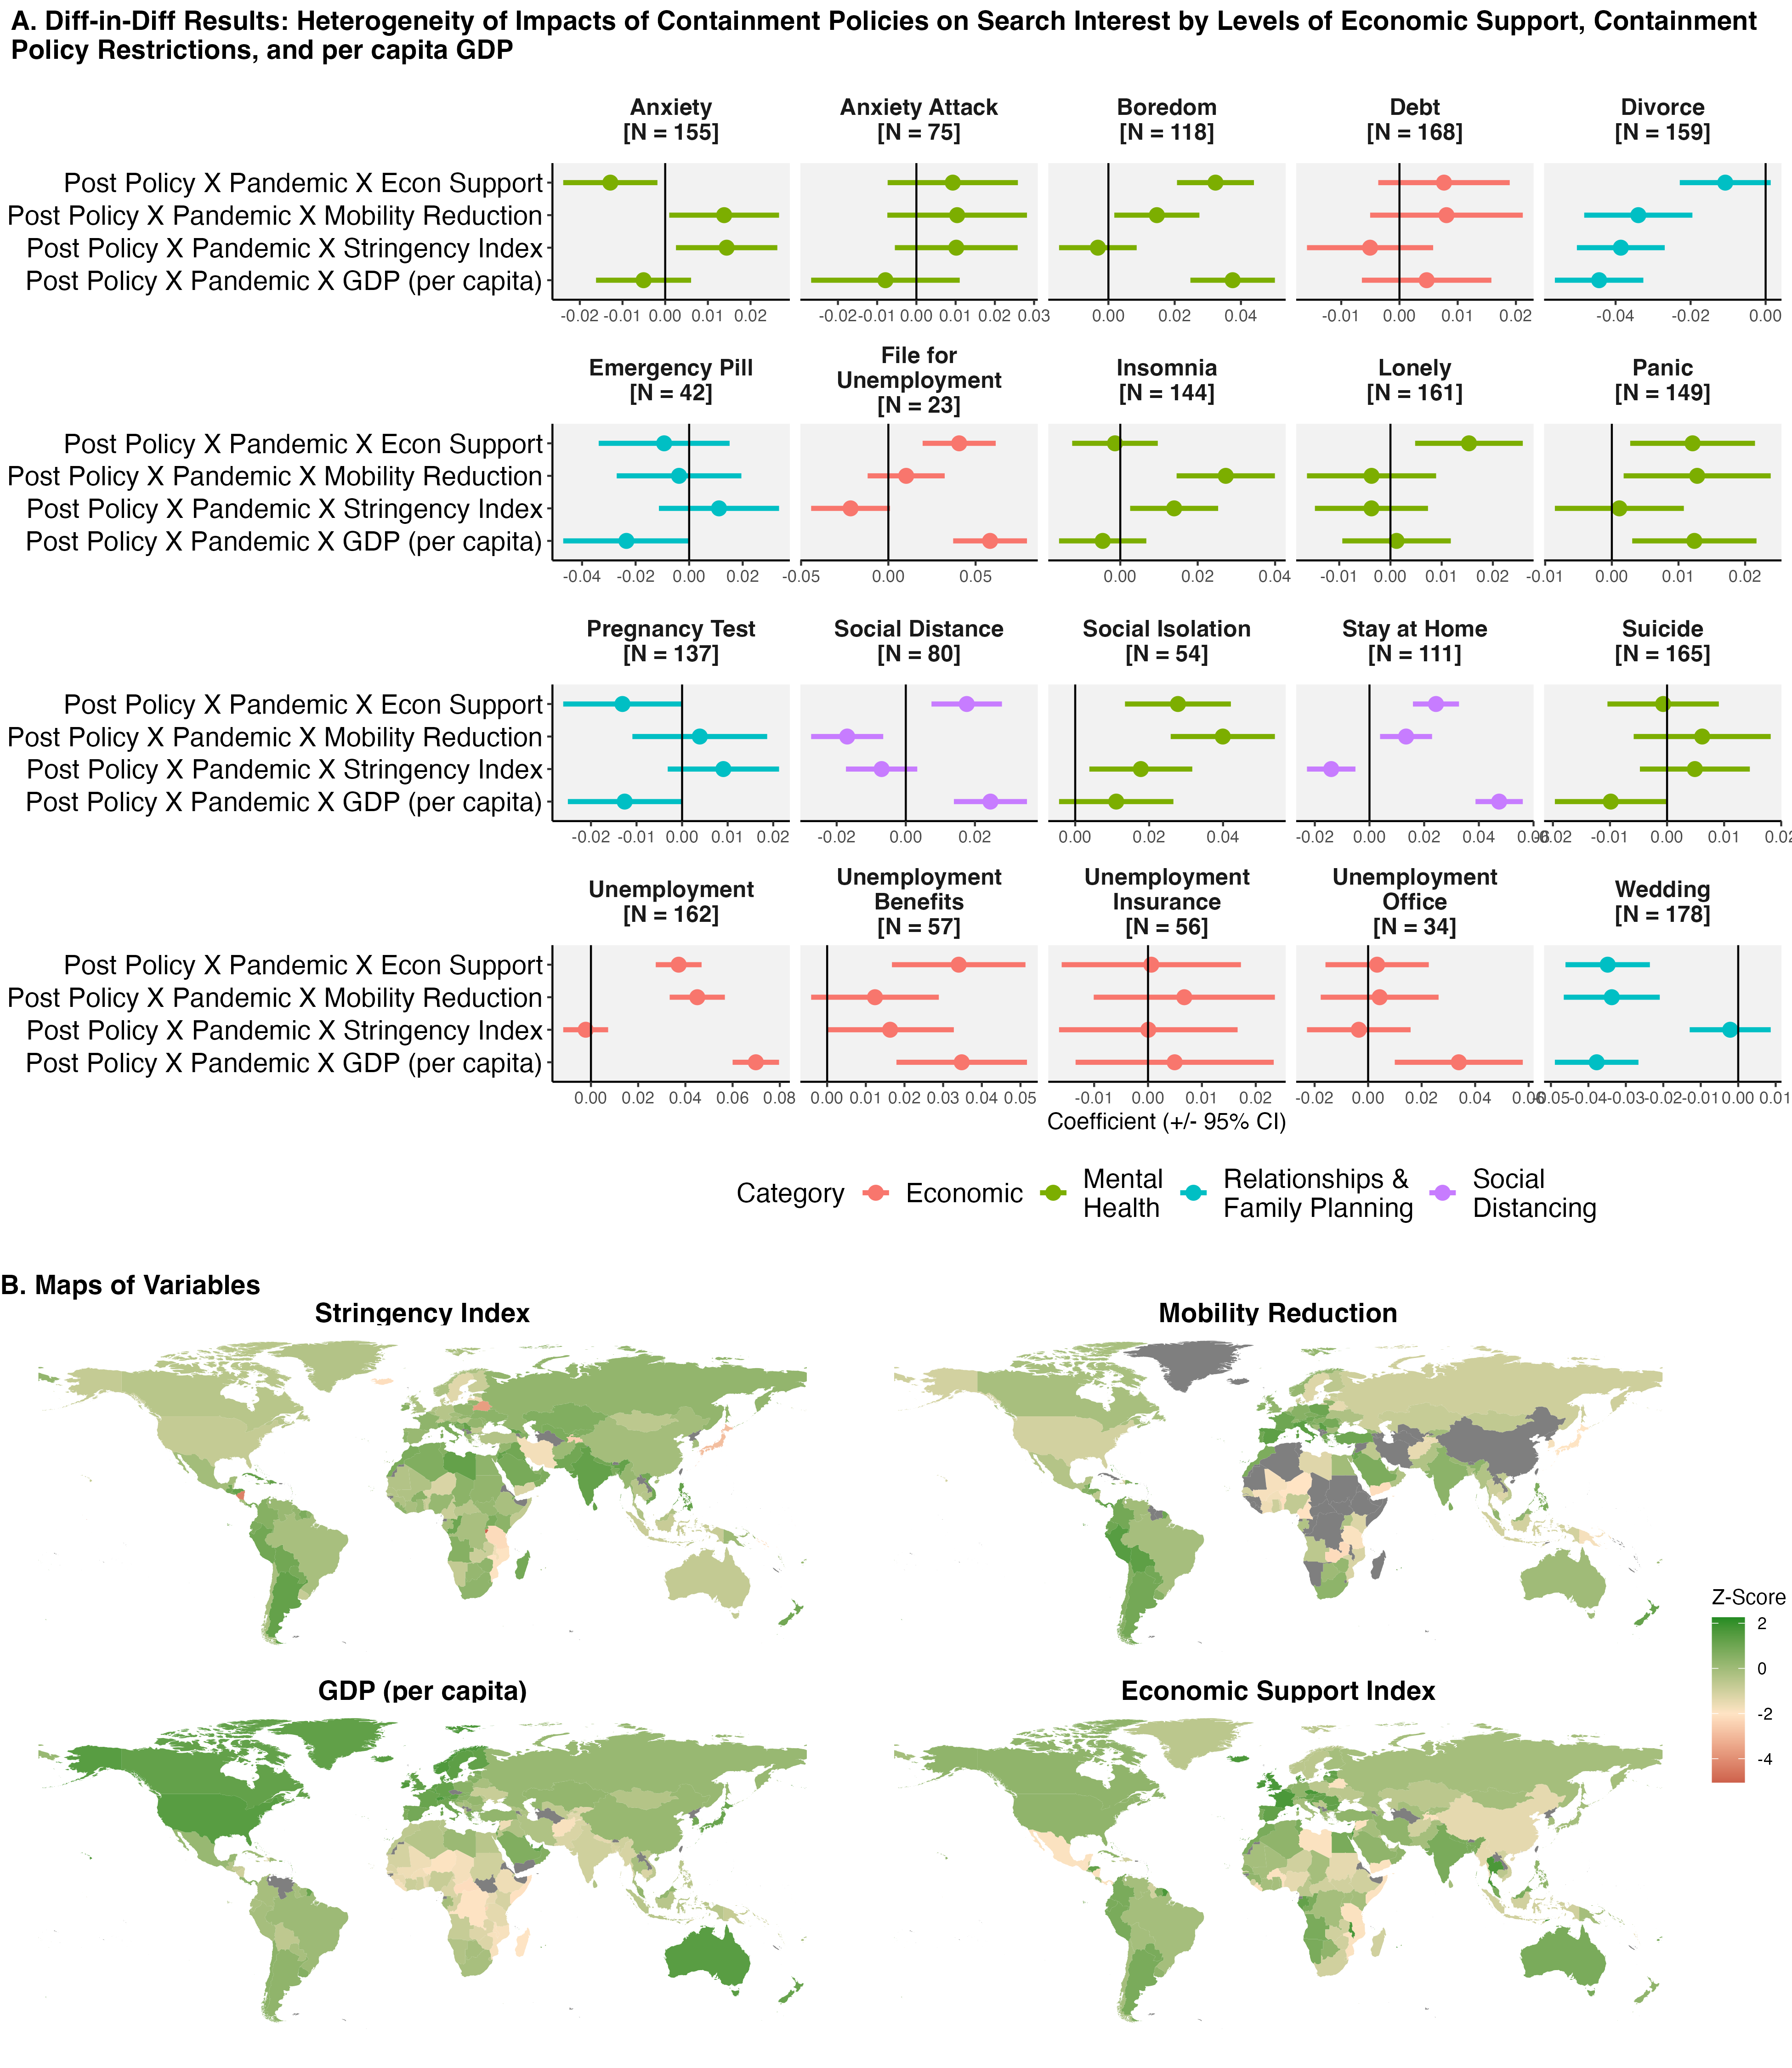
\includegraphics[width=0.85\textwidth]{figures/did_interact_map_90.png}
    \caption{\textcolor{black}{Association of COVID-19 policies with search interest: difference-in-differences results that explore heterogeneity of results} across containment policy restrictiveness, economic support, and GDP per capita. Each coefficient comes from a separate regression. The stringency index comes from the University of Oxford COVID-19 Government Response tracker, a composite measure of the restrictiveness of policy measures. Mobility reduction comes from Google COVID-19 Community Mobility Reports, which measure the percent change in mobility relative to pre-pandemic levels. Per capita GDP comes from the World Bank's World Development Indicators; we use log per capita GDP. The Economic Support index from the Oxford COVID-19 Government Response tracker, which measures the extent of economic support across metrics such as income support and debt relief. We standardize all variables into z-scores---having a mean of zero and standard deviation of one. \textcolor{black}{`N' indicates the number of countries with available data. Maps produced using R, version 4.2.2 (\url{https://www.r-project.org/}); data for country boundaries come from Natural Earth (\url{https://www.naturalearthdata.com/}).}}    
    \label{fig:did_interact_map_90}
\end{figure*}

\begin{figure*}[t]
    \centering
    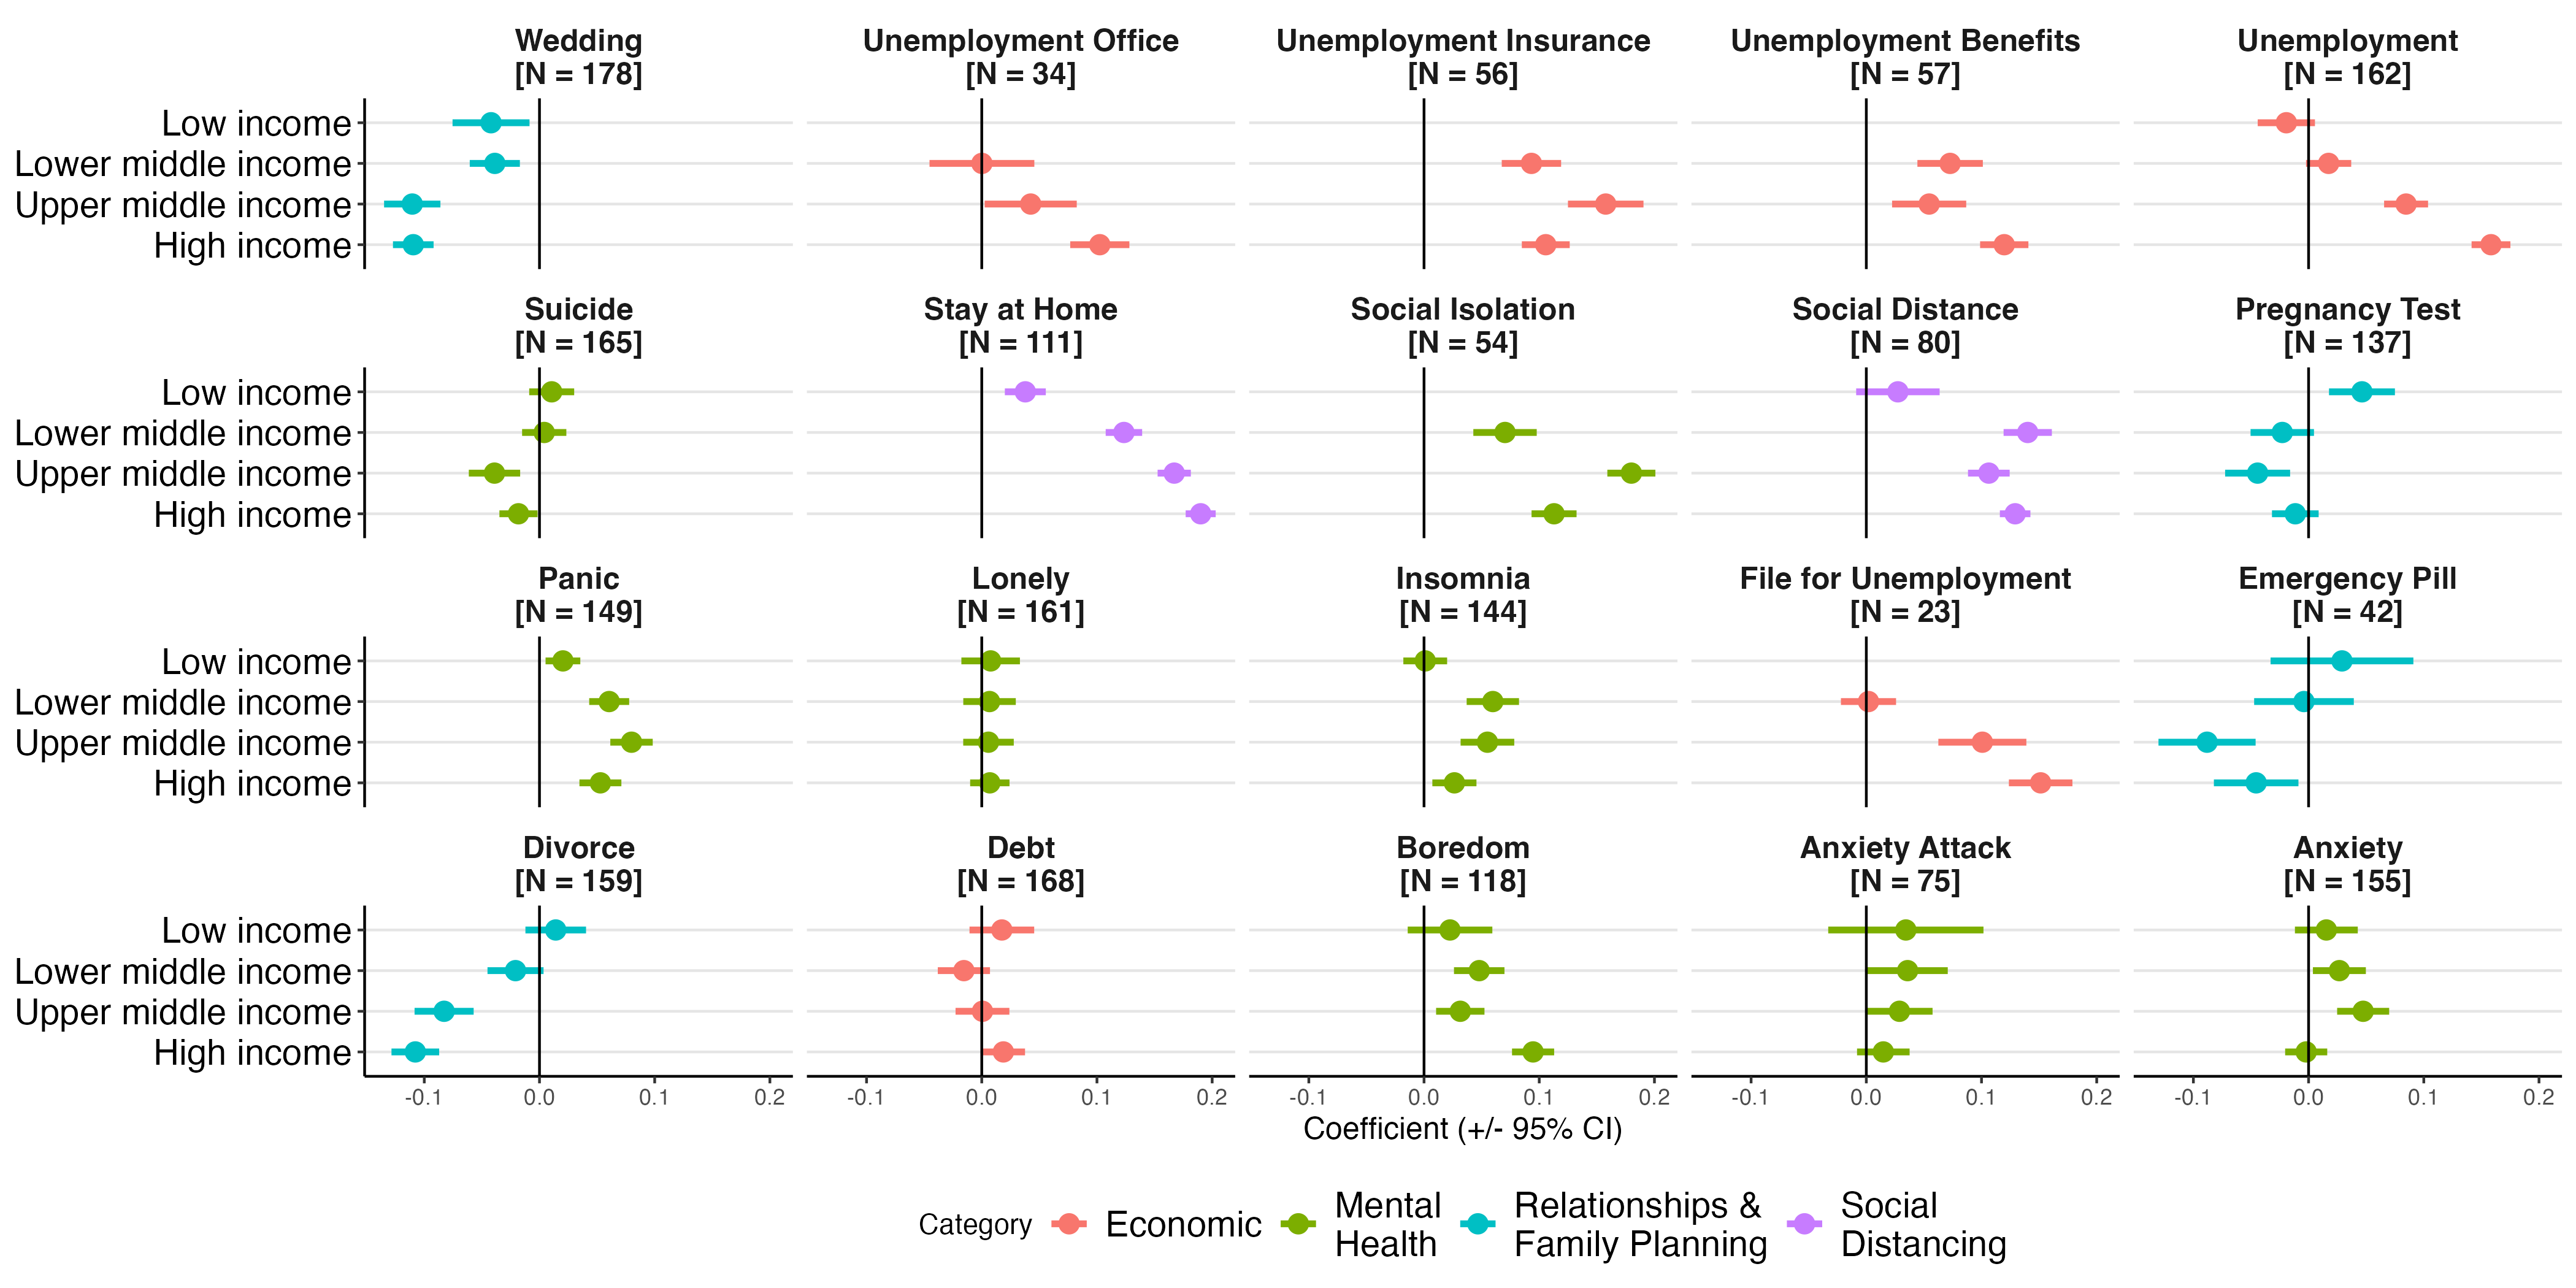
\includegraphics[width=0.85\textwidth]{figures/did_income_90.png}
    \caption{\textcolor{black}{Association of COVID-19 policies and} search interest: difference-in-difference results pooling countries by income level. Point estimates and 95\% confidence intervals are shown. \textcolor{black}{`N' indicates the number of countries with available data.}}
    \label{fig:did_income_90}
\end{figure*}

\end{document}


















































